\documentclass[]{article}

% Imported Packages
%------------------------------------------------------------------------------
\usepackage{amssymb}
\usepackage{amstext}
\usepackage{amsthm}
\usepackage{amsmath}
\usepackage{enumerate}
\usepackage{fancyhdr}
\usepackage[margin=1in]{geometry}
\usepackage{graphicx}
%\usepackage{extarrows}
%\usepackage{setspace}
%\usepackage{xcolor}
\usepackage{color}
\usepackage{parskip}
%------------------------------------------------------------------------------

% Header and Footer
%------------------------------------------------------------------------------
\pagestyle{plain}  
\renewcommand\headrulewidth{0.4pt}                                      
\renewcommand\footrulewidth{0.4pt}                                    
%------------------------------------------------------------------------------

% Title Details
%------------------------------------------------------------------------------
\title{Deliverable \#1 Template : Software Requirement Specification (SRS)}
\author{SE 3A04: Software Design II -- Large System Design}
\date{}
                            
%------------------------------------------------------------------------------

% Document
%------------------------------------------------------------------------------
\begin{document}

\maketitle	
\noindent{\bf Tutorial Number:} T03\\
{\bf Group Number:} G8 \\
{\bf Group Members:} 
\begin{itemize}
	\item Adam Mak
	\item Eric Chen
	\item Justin Ho
	\item Ahmad Hamadi
	\item Kevin Ishak
	\item Jonathan Jiang
\end{itemize}

\section*{IMPORTANT NOTES}
\begin{itemize}
	\item Be sure to include all sections of the template in your document regardless whether you have something to write for each or not
	\begin{itemize}
		\item If you do not have anything to write in a section, indicate this by the \emph{N/A}, \emph{void}, \emph{none}, etc.
	\end{itemize}
	\item Uniquely number each of your requirements for easy identification and cross-referencing
	\item Highlight terms that are defined in Section~1.3 (\textbf{Definitions, Acronyms, and Abbreviations}) with \textbf{bold}, \emph{italic} or \underline{underline}
	\item For Deliverable 1, please highlight, in some fashion, all (you may have more than one) creative and innovative features. Your creative and innovative features will generally be described in Section~2.2 (\textbf{Product Functions}), but it will depend on the type of creative or innovative features you are including.
\end{itemize}

\newpage
\section{Introduction}
\label{sec:introduction}
% Begin Section

\subsection{Purpose}
\label{sub:purpose}
% Begin SubSection
The purpose of this SRS is to define the functionality and characteristics that the carpool app should have. It should provide a detailed overview of all the processes and systems that needs to be present in the final product. It describes the system and user interaction with the application. Intended audience for the SRS:
\begin{itemize}
	\item Developers
	\item UI/UX Designers
	\item Product Managers
	\item Engineers
	\item System Architects
	\item Quality Assurance Testers
\end{itemize}
% End SubSection

\subsection{Scope}
\label{sub:scope}
% Begin SubSection
The software product is a taxi carpool service. It will provide a communication environment for passengers to carpool via taxis. This service is not meant to be replacement for taxi services (i.e. Uber-like services).

The objective of the software (local taxi system) being implemented is to transport users from one destination to another using a carpool method. This software allows user to enter a destination along with some optional search criteria that they want to arrive at. The software will then match the user with a taxi nearby which may or may not carry other individuals who are travelling in the same general direction. This benefits both the users, taxi driver as well as the environment by as it helps reduce costs, whether it be the fare for the ride or the reduction in environmental pollutants by the means of carpooling.

There are no higher-level specifications that exist, thus, any lower-level specifications must be consistent with this document, as it is the highest-level specification.
% End SubSection

\subsection{Definitions, Acronyms, and Abbreviations}
\label{sub:definitions_acronyms_and_abbreviations}
% Begin SubSection
\begin{center} \begin{tabular} {|c|p{35em}|}
	\hline
	\textbf{Abbreviation/Acronym} & \textbf{Definition} \\
	\hline \hline
	API & Application Programming Interface \\
	\hline
	Carpool & To collectively share a ride (either to help reduce the cost of transit or as an act of being more environmentally “green”) \\
	\hline
	DBMS & Database Management System \\
	\hline
	GoPlay Store & The default Android distribution platform \\
	\hline
	SMS & Software Requirements Specification \\
	\hline
	SRS & Simple Message Service \\
	\hline
\end{tabular} \end{center}
% End SubSection

\subsection{References}
\label{sub:references}
% Begin SubSection
\begin{itemize}
	\item Provide a complete list of all documents referenced elsewhere in the SRS.
	\item Identify each document by title, report number (if applicable), date, and publishing organization.
	\item Specify the sources from which the references can be obtained.
	\item Order this list in some sensible manner (alphabetical by author, or something else that makes more sense).
\end{itemize}
% End SubSection

\subsection{Overview}
\label{sub:overview}
% Begin SubSection
In the order of occurrence, the remainder of the SRS contains an overview of the system, which includes product perspective, product functions, user characteristics, constraints, and dependencies. The SRS will have a descriptive model, which will be represented visually in the form of a use-case diagram. Furthermore, the document also includes various system-specific requirements which are consist of functional and non-functional requirements.  Finally, at the end of the document, there is a record which represents the division of labour of all contributors to the project.
% End SubSection

% End Section

\section{Overall Product Description}
\label{sec:overall_description}
% Begin Section

\subsection{Product Perspective}
\label{sub:product_perspective}
% Begin SubSection
The carpool app product is independent and self-contained, as it does not build upon any existing products/applications. However, the standalone system uses and owns interfaces to and from external systems, such as hardware, users, databases, and other API's, to provide essential functionality to the app. Figure \ref{fig:blockdiagram} shows how these external systems will interact in a block diagram.

The carpooling app is developed for Android devices, providing users owning these devices with easy access to this service. Also, the app's user interface interacts with an Android device to allow users to see information and interact with the application through a touchscreen.

The app sends and receives data from a database that stores information about users, rides, route information, and other related data. This is managed by a DBMS.

The carpooling app uses the Google Map API to provide maps and location-related services such as route planning and estimating travel times. The API provides information about the locations of users and destinations, as well as real-time traffic data, to help drivers make more informed decisions about their routes.

To protect sensitive information such as passwords, payment information, transmitted messages, and other confidential data, the carpooling app uses a cryptosystem to encrypt this information before it is stored in the DBMS. When the data is needed, it is decrypted and used by the app. This ensures that information is protected from unauthorized access.

The carpooling app uses SMS functionality to provide communication between users to provide updates, confirm ride details, and more. For instance, when a ride is requested, the app may send a message to the driver to notify them of the request, and then another message to the passenger to confirm the ride details.

\begin{figure}[h!]
	\centering
	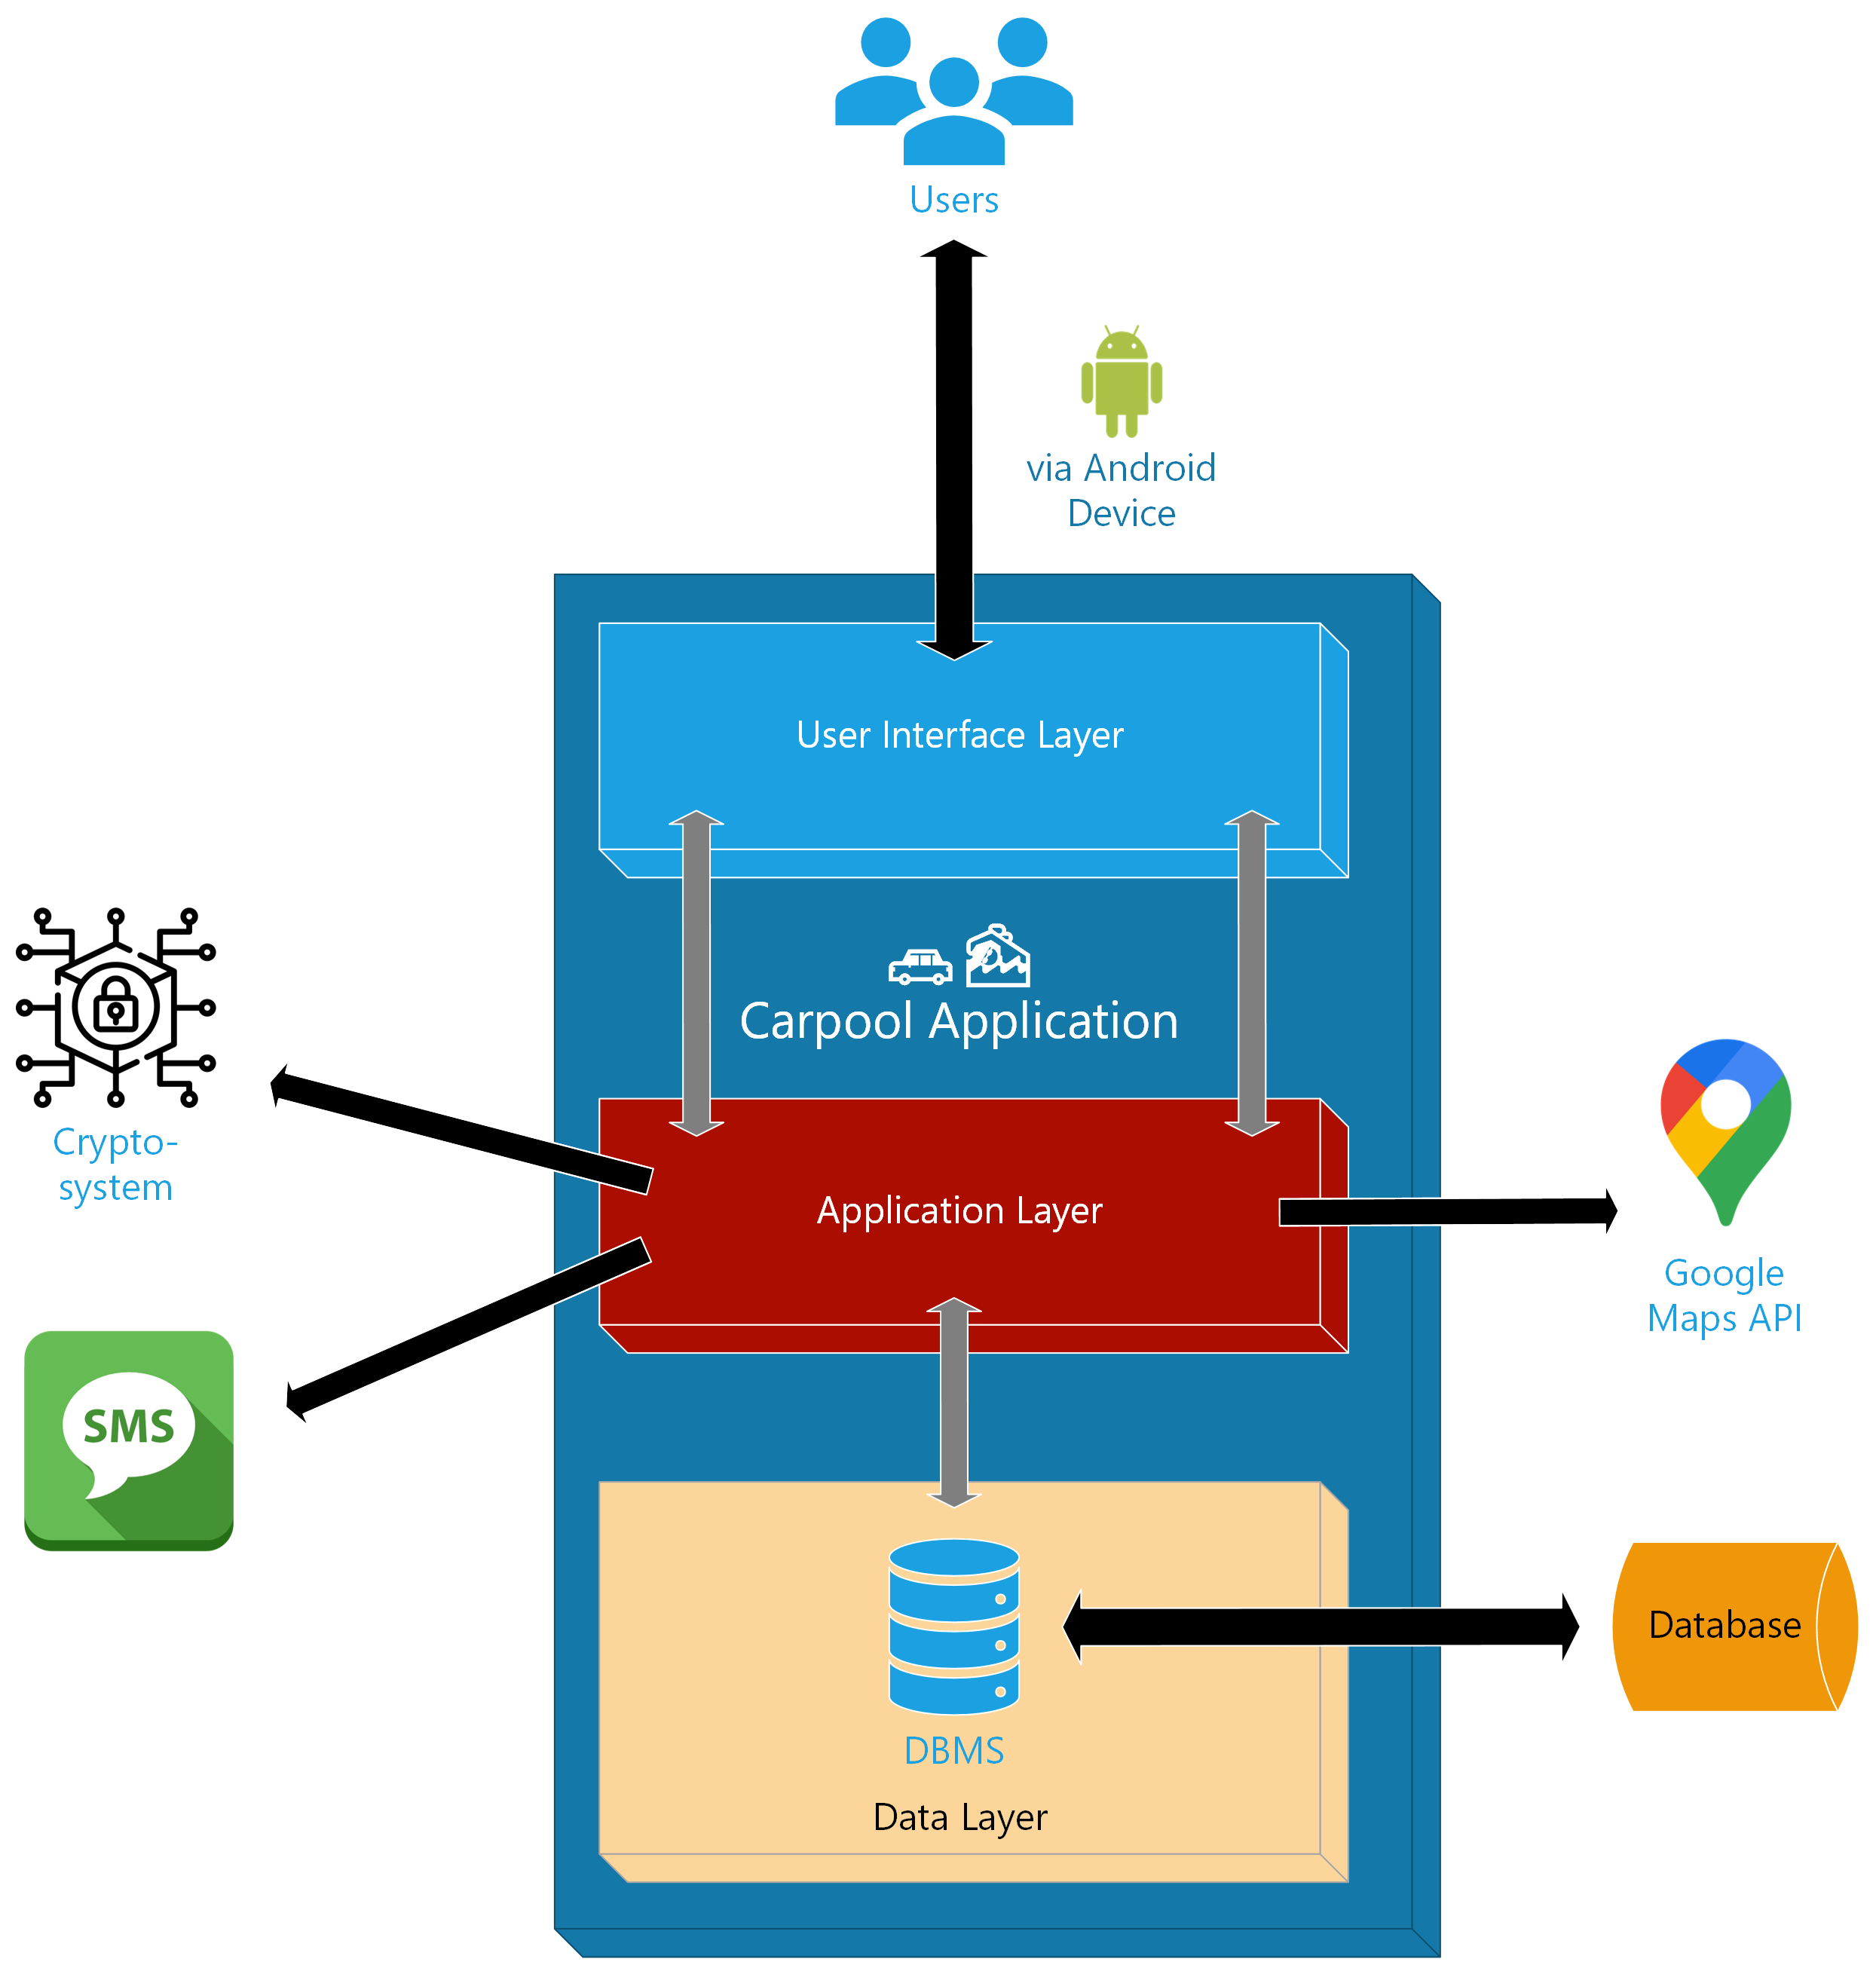
\includegraphics[width=30em]{ProductPerspectiveBlockDiagram.png}
	\caption{A block diagram showing the major layers of the carpooling application, interconnections, and external interfaces.}
	\label{fig:blockdiagram}
\end{figure}
% End SubSection

\subsection{Product Functions}
\label{sub:product_functions}
% Begin SubSection
\begin{itemize}
	\item App should compare carpool price with non carpool price and display the money saved as a point system.
	\item App should allow carpoolers to setup/join other carpoolers using the app.
	\item When requesting a carpool, carpoolers should be able to filter through different travel options (i.e. sort by closest cab/highest rated cab driver). The app should return a list of cab options according to the specification.
	\item Carpoolers looking to set up a carpool should be able to input the taxi ID , destination, maximum number of other carpoolers,  as well as potential auxiliary information. They system should post this info and allow other carpoolers to join.
	\item Users should be able to create and delete accounts, which the system should store.
	\item The system should check if a user that wants to request/setup a carpool is a registered user. It should reject unregistered users.
\end{itemize}
% End SubSection

\subsection{User Characteristics}
\label{sub:user_characteristics}
% Begin SubSection
Users include both passengers and drivers, of which age and education level may vary. The users of the product are expected to have a basic knowledge of technology and are familiar with smartphones, which the app is developed for.	 
% End SubSection

\subsection{Constraints}
\label{sub:constraints}
% Begin SubSection
\begin{itemize}
	\item Legal and regulatory restrictions: The developer needs to ensure that the application complies with the local laws and regulations.
	\item Technical limitations: The developer may face limitations with regards to the technology used to build the application, such as compatibility with different platforms, scalability, and security.
	\item Competition: They need to differentiate their product and offer unique features.
	\item Budget and resources: The availability of financial and human resources can impact the scope and timeline of the project.
\end{itemize}
% End SubSection

\subsection{Assumptions and Dependencies}
\label{sub:assumptions_and_dependencies}
% Begin SubSection
The carpool app will be available for installation/download through the Apple and Google Play store for users to use. It is assumed that Apple/Google Play will streamline our app upon the necessary guidelines being met (I.e., Safety, Privacy, Performance, Business, Design, Legal).

It is assumed that the Google Maps API will be available to use with an 100\% uptime which our carpool app will utilize to plan its routes and navigate users around cities. If the Google Maps API, for some extenuating circumstances, is unable to provide the services for route navigation, then another GIS API system may have to be utilized (e.g., OpenLayers, ESRI, etc…).

A primary telecommunication company will be managing the SMS traffic of the carpool app as the app makes use of SMS functionality to inform users about the status of their ride. If for some reason, any of the telecommunication companies listed within this SRS document disbands, terminates the contract or breach some sort of confidentiality between both parties, and/or something similar in nature, then the SRS might have to change accordingly to fill up the vacant SMS management company.

It is assumed that the carpool app will be systematically be calculating the cost of the trip per person on a reduced per mileage basis. 
% End SubSection

\subsection{Apportioning of Requirements}
\label{sub:apportioning_of_requirements}
% Begin SubSection
The following requirements are usually delayed until later versions to meet the initial launch deadline and budget, or to focus on delivering the most valuable features to users first.

\begin{enumerate}
	\item Advanced features: These are features that are not essential to the core functionality of the app, but can be added later as the app evolves.
	\begin{itemize}
		\item[-] For example, an in-app tipping feature, or integration with a rewards program. 
	\end{itemize}
	\item Non-critical performance optimizations: Improving the app's performance can be a continuous process, and some optimizations can be deferred until later versions.
	\begin{itemize}
		\item[-] For example, optimizations that improve the app's speed, reliability or efficiency, but are not essential to its basic functionality.  
	\end{itemize}
	\item Complex user interfaces: Advanced user interfaces can be time-consuming to develop and may be deferred in favor of a simpler interface in the initial release. 
	\begin{itemize}
		\item[-] For example, a more sophisticated design that includes augmented reality, or a chatbot interface.  
	\end{itemize}
	\item Integrations with third-party systems: Integrating the app with other systems can be a significant effort, and this work may be deferred until later versions. 
	\begin{itemize}
		\item[-] For example, integration with a payment system, or with a local transit system. 
	\end{itemize}
	\item Support for older platforms: Supporting older platforms can be time-consuming, and this work may be deferred until later versions or only supported for critical security and bug fixes.
	\begin{itemize}
		\item[-] For example, supporting older versions of the iOS or Android operating systems. 
	\end{itemize}
\end{enumerate}

\noindent It is important to prioritize the most critical requirements, such as the core functionality of booking a ride, and ensuring that the app is easy to use. Other requirements can be deferred until future versions to meet the initial launch deadline and budget. 
% End SubSection

% End Section
\section{Use Case Diagram}
\label{sec:use_case_diagram}
% Begin Section
\begin{itemize}
	\item Provide the use case diagram for the system being developed.
	\item You do not need to provide the textual description of any of the use cases here (these will be specified under "Highlights of Functional Requirements").
%	\item Provide \emph{one} use case diagram for the most important Business Event.
%	\item The text of all use cases will be specified under "Highlights of Functional Requirements"
\end{itemize}
%In this section, select the most important Business Event that your system responds to and give its use case diagram.  Only one use case diagram is needed.  Give a brief textual description of the use case without repeating what is in the scenarios of the corresponding Business Event.

%
%
%
%This section should provide a use case diagram for your application. 
%\begin{enumerate}[a)]
%	\item Each use case appearing in the diagram should be accompanied by a text description. 
%\end{enumerate}
%% End Section

\section{Highlights of Functional Requirements}
\label{sec:functional_requirements}
% Begin Section
\begin{itemize}
	\item Specify all use cases (or other scenarios triggered by other events), organized by Business Event. 
	\item For each Business Event, show the scenario from every Viewpoint. You should have the same set of Viewpoints across all Business Events. If a Viewpoint doesn't participate, write N/A so we know you considered it still. You can choose how to present this - keep in mind it should be easy to follow. 
	\item At the end, combine them all into a Global Scenario.
	%\item Specify the "use cases" (or other triggering events) organized by Business Event. (The Global Scenario is what you might think of as a use case). Be sure to consider Business Events that aren't just triggered by users with goals (e.g. something happens in the environment that your system needs to respond to)
	\item Your focus should be on what the system needs to do, not how to do it. Specify it in enough detail that it clearly specifies what needs to be accomplished, but not so detailed that you start programming or making design decisions.
	\item Keep the length of each use case (Global Scenario) manageable. If it's getting too long, split into sub-cases.
	\item You are \emph{not} specifying a complete and consistent set of functional requirements here. (i.e. you are providing them in the form of use cases/global scenarios, not a refined list). For the purpose of this project, you do not need to reduce them to a list; the global scenarios format is all you need.
	\item Red text below is just to highlight where you need to insert a scenario - don't actually write it all in red.
\end{itemize}

\noindent {\bf Main Business Events:} List out all the main business events you are presenting. If you sub-divided into smaller ones, you don't need to include the smaller ones in this list.\\

\noindent {\bf Viewpoints:} List out all the viewpoints you will be considering.\\

\noindent {\bf Interpretation:} Specify any liberties you took in interpreting business events, if necessary.\\

\begin{enumerate}[{\bf BE1.}]
	\item Business Event Name \#1
		\begin{enumerate}[{\bf VP1.}]
			\item Viewpoint Name \#1 \\
				\textcolor{red}{Insert Scenario Here}
			\item Viewpoint Name \#2 \\
				\textcolor{red}{Insert Scenario Here}
		\end{enumerate}
		{\bf Global Scenario:}\\
		\textcolor{red}{Insert Scenario Here}
	\item Business Event Name \#2
	\begin{enumerate}[{\bf VP1.}]
		\item Viewpoint Name \#1 \\
		\textcolor{red}{Insert Scenario Here}
		\item Viewpoint Name \#2 \\
		\textcolor{red}{Insert Scenario Here}
	\end{enumerate}
	{\bf Global Scenario:}\\
	\textcolor{red}{Insert Scenario Here}
\end{enumerate}

%	Below, we organize by Business Event.
%	\begin{enumerate}[{BE}1.]
%		\item Business Event name
%		\begin{enumerate}[{VP1}.1]
%			\item Viewpoint name \newline
%			\noindent\fbox{%
%				\parbox{0.5\textwidth}{%
%					\begin{itemize}
%						\item {\bf $S_{1}$:} Initial response of the system to the Business Event
%						\item {\bf $E_{1}$:}  Reaction of the environment to $S_{1}$
%						\item {\bf $S_{2}$:}  Response of the system to $E_{1}$
%						\item {\bf $E_{2}$:}  Reaction of the environment to $S_{2}$
%						\item[] $\cdots$
%						\item {\bf $S_{n}$:}  Response of the system to $E_{(n-1)}$
%						\item {\bf $E_{n}$:}  Reaction of the environment to $E_{(n-1)}$
%						\item {\bf $S_{(n+1)}$:} Final response of the system concluding its function regarding the Business Event
%					\end{itemize}
%				}%
%			}
%			\item Viewpoint name\newline
%			\noindent\fbox{%
%				\parbox{0.5\textwidth}{%
%					\begin{itemize}
%						\item {\bf $S_{1}$:} Initial response of the system to the Business Event
%						\item {\bf $E_{1}$:}  Reaction of the environment to $S_{1}$
%						\item {\bf $S_{2}$:}  Response of the system to $E_{1}$
%						\item {\bf $E_{2}$:}  Reaction of the environment to $S_{2}$
%						\item[] $\cdots$
%						\item {\bf $S_{k}$:}  Response of the system to $E_{(k-1)}$
%						\item {\bf $E_{k}$:}  Reaction of the environment to $E_{(k-1)}$
%						\item {\bf $S_{(k+1)}$:} Final response of the system concluding its function regarding the Business Event
%					\end{itemize}
%				}%
%			}
%			\item \dots
%			\item \dots
%			\item \dots
%			\item[\dots]
%		\end{enumerate}	
%		\item[] {\bf Global Scenario of {\it Business Event Name}:} It is the scenario corresponding to the integration of all the above scenarios from the different Viewpoints of the Business Event BE1.\newline
%		\noindent\fbox{%
%			\parbox{0.5\textwidth}{%
%				\begin{itemize}
%					\item {\bf $S_{1}$:} Initial response of the system to the Business Event
%					\item {\bf $E_{1}$:}  Reaction of the environment to $S_{1}$
%					\item {\bf $S_{2}$:}  Response of the system to $E_{1}$
%					\item {\bf $E_{2}$:}  Reaction of the environment to $S_{2}$
%					\item[] $\cdots$
%					\item {\bf $S_{m}$:}  Response of the system to $E_{(m-1)}$
%					\item {\bf $E_{m}$:}  Reaction of the environment to $E_{(m-1)}$
%					\item {\bf $S_{(m+1)}$:} Final response of the system concluding its function regarding the Business Event
%				\end{itemize}
%			}%
%		}	
%		%\end{enumerate}
%		\item Business Event name
%		\begin{enumerate}[{VP1}.1]
%			\item Viewpoint name \newline
%			\noindent\fbox{%
%				\parbox{0.5\textwidth}{%
%					\begin{itemize}
%						\item {\bf $S_{1}$:} Initial response of the system to the Business Event
%						\item {\bf $E_{1}$:}  Reaction of the environment to $S_{1}$
%						\item {\bf $S_{2}$:}  Response of the system to $E_{1}$
%						\item {\bf $E_{2}$:}  Reaction of the environment to $S_{2}$
%						\item[] $\cdots$
%						\item {\bf $S_{n'}$:}  Response of the system to $E_{(n'-1)}$
%						\item {\bf $E_{n'}$:}  Reaction of the environment to $E_{(n'-1)}$
%						\item {\bf $S_{(n'+1)}$:} Final response of the system concluding its function regarding the Business Event
%					\end{itemize}
%				}%
%			}
%			\item Viewpoint name\newline
%			\noindent\fbox{%
%				\parbox{0.5\textwidth}{%
%					\begin{itemize}
%						\item {\bf $S_{1}$:} Initial response of the system to the Business Event
%						\item {\bf $E_{1}$:}  Reaction of the environment to $S_{1}$
%						\item {\bf $S_{2}$:}  Response of the system to $E_{1}$
%						\item {\bf $E_{2}$:}  Reaction of the environment to $S_{2}$
%						\item[] $\cdots$
%						\item {\bf $S_{k'}$:}  Response of the system to $E_{(k'-1)}$
%						\item {\bf $E_{k'}$:}  Reaction of the environment to $E_{(k'-1)}$
%						\item {\bf $S_{(k'+1)}$:} Final response of the system concluding its function regarding the Business Event
%					\end{itemize}
%				}%
%			}
%			\item \dots
%			\item \dots
%			\item \dots
%			\item[\dots]
%		\end{enumerate}	
%		\item[] {\bf Global Scenario of {\it Business Event Name}:} It is the scenario corresponding to the integration of all the above scenarios from the different Viewpoints of the Business Event BE2.\newline
%		\noindent\fbox{%
%			\parbox{0.5\textwidth}{%
%				\begin{itemize}
%					\item {\bf $S_{1}$:} Initial response of the system to the Business Event
%					\item {\bf $E_{1}$:}  Reaction of the environment to $S_{1}$
%					\item {\bf $S_{2}$:}  Response of the system to $E_{1}$
%					\item {\bf $E_{2}$:}  Reaction of the environment to $S_{2}$
%					\item[] $\cdots$
%					\item {\bf $S_{m'}$:}  Response of the system to $E_{(m'-1)}$
%					\item {\bf $E_{m'}$:}  Reaction of the environment to $E_{(m'-1)}$
%					\item {\bf $S_{(m'+1)}$:} Final response of the system concluding its function regarding the Business Event
%				\end{itemize}
%			}%
%		}		
%	\end{enumerate}

%End Section

\section{Non-Functional Requirements}
\label{sec:non-functional_requirements}


\begin{itemize}
	\item For each non-functional requirement, provide a justification/rationale for it.\\
	{\bf Example:} \\
	SC1. \emph{The device should not explode in a customer’s pocket.}\\
	{\bf Rationale:} Other companies have had issues with the batteries they used in their phones randomly exploding [insert citation]. This causes a safety issue, as the phone is often carried in a person's hand or pocket.	
	\item If you need to make a guess because you couldn't really talk to stakeholders, you can say "We imagined stakeholders would want...because..."
	\item Each requirement should have a unique label/number for it.
	\item In the list below, if a particular section doesn't apply, just write N/A so we know you considered it.
\end{itemize}

% Begin Section
\subsection{Look and Feel Requirements}
\label{sub:look_and_feel_requirements}
% Begin SubSection

\subsubsection{Appearance Requirements}
\label{ssub:appearance_requirements}
% Begin SubSubSection
\begin{enumerate}[{LF-A}1. ]
	\item 
\end{enumerate}
% End SubSubSection

\subsubsection{Style Requirements}
\label{ssub:style_requirements}
% Begin SubSubSection
\begin{enumerate}[{LF-S}1. ]
	\item 
\end{enumerate}
% End SubSubSection

% End SubSection

\subsection{Usability and Humanity Requirements}
\label{sub:usability_and_humanity_requirements}
% Begin SubSection

\subsubsection{Ease of Use Requirements}
\label{ssub:ease_of_use_requirements}
% Begin SubSubSection
\begin{enumerate}[{UH-EOU}1. ]
	\item 
\end{enumerate}
% End SubSubSection

\subsubsection{Personalization and Internationalization Requirements}
\label{ssub:personalization_and_internationalization_requirements}
% Begin SubSubSection
\begin{enumerate}[{UH-PI}1. ]
	\item 
\end{enumerate}
% End SubSubSection

\subsubsection{Learning Requirements}
\label{ssub:learning_requirements}
% Begin SubSubSection
\begin{enumerate}[{UH-L}1. ]
	\item 
\end{enumerate}
% End SubSubSection

\subsubsection{Understandability and Politeness Requirements}
\label{ssub:understandability_and_politeness_requirements}
% Begin SubSubSection
\begin{enumerate}[{UH-UP}1. ]
	\item 
\end{enumerate}
% End SubSubSection

\subsubsection{Accessibility Requirements}
\label{ssub:accessibility_requirements}
% Begin SubSubSection
\begin{enumerate}[{UH-A}1. ]
	\item 
\end{enumerate}
% End SubSubSection

% End SubSection

\subsection{Performance Requirements}
\label{sub:performance_requirements}
% Begin SubSection

\subsubsection{Speed and Latency Requirements}
\label{ssub:speed_and_latency_requirements}
% Begin SubSubSection
\begin{enumerate}[{PR-SL}1. ]
	\item 
\end{enumerate}
% End SubSubSection

\subsubsection{Safety-Critical Requirements}
\label{ssub:safety_critical_requirements}
% Begin SubSubSection
\begin{enumerate}[{PR-SC}1. ]
	\item 
\end{enumerate}
% End SubSubSection

\subsubsection{Precision or Accuracy Requirements}
\label{ssub:precision_or_accuracy_requirements}
% Begin SubSubSection
\begin{enumerate}[{PR-PA}1. ]
	\item 
\end{enumerate}
% End SubSubSection

\subsubsection{Reliability and Availability Requirements}
\label{ssub:reliability_and_availability_requirements}
% Begin SubSubSection
\begin{enumerate}[{PR-RA}1. ]
	\item 
\end{enumerate}
% End SubSubSection

\subsubsection{Robustness or Fault-Tolerance Requirements}
\label{ssub:robustness_or_fault_tolerance_requirements}
% Begin SubSubSection
\begin{enumerate}[{PR-RFT}1. ]
	\item 
\end{enumerate}
% End SubSubSection

\subsubsection{Capacity Requirements}
\label{ssub:capacity_requirements}
% Begin SubSubSection
\begin{enumerate}[{PR-C}1. ]
	\item 
\end{enumerate}
% End SubSubSection

\subsubsection{Scalability or Extensibility Requirements}
\label{ssub:scalability_or_extensibility_requirements}
% Begin SubSubSection
\begin{enumerate}[{PR-SE}1. ]
	\item 
\end{enumerate}
% End SubSubSection

\subsubsection{Longevity Requirements}
\label{ssub:longevity_requirements}
% Begin SubSubSection
\begin{enumerate}[{PR-L}1. ]
	\item 
\end{enumerate}
% End SubSubSection

% End SubSection

\subsection{Operational and Environmental Requirements}
\label{sub:operational_and_environmental_requirements}
% Begin SubSection

\subsubsection{Expected Physical Environment}
\label{ssub:expected_physical_environment}
% Begin SubSubSection
\begin{enumerate}[{OE-EPE}1. ]
	\item 
\end{enumerate}
% End SubSubSection

\subsubsection{Requirements for Interfacing with Adjacent Systems}
\label{ssub:requirements_for_interfacing_with_adjacent_systems}
% Begin SubSubSection
\begin{enumerate}[{OE-IA}1. ]
	\item 
\end{enumerate}
% End SubSubSection

\subsubsection{Productization Requirements}
\label{ssub:productization_requirements}
% Begin SubSubSection
\begin{enumerate}[{OE-P}1. ]
	\item 
\end{enumerate}
% End SubSubSection

\subsubsection{Release Requirements}
\label{ssub:release_requirements}
% Begin SubSubSection
\begin{enumerate}[{OE-R}1. ]
	\item 
\end{enumerate}
% End SubSubSection

% End SubSection

\subsection{Maintainability and Support Requirements}
\label{sub:maintainability_and_support_requirements}
% Begin SubSection

\subsubsection{Maintenance Requirements}
\label{ssub:maintenance_requirements}
% Begin SubSubSection
\begin{enumerate}[{MS-M}1. ]
	\item 
\end{enumerate}
% End SubSubSection

\subsubsection{Supportability Requirements}
\label{ssub:supportability_requirements}
% Begin SubSubSection
\begin{enumerate}[{MS-S}1. ]
	\item 
\end{enumerate}
% End SubSubSection

\subsubsection{Adaptability Requirements}
\label{ssub:adaptability_requirements}
% Begin SubSubSection
\begin{enumerate}[{MS-A}1. ]
	\item 
\end{enumerate}
% End SubSubSection

% End SubSection

\subsection{Security Requirements}
\label{sub:security_requirements}
% Begin SubSection

\subsubsection{Access Requirements}
\label{ssub:access_requirements}
% Begin SubSubSection
\begin{enumerate}[{SR-AC}1. ]
	\item 
\end{enumerate}
% End SubSubSection

\subsubsection{Integrity Requirements}
\label{ssub:integrity_requirements}
% Begin SubSubSection
\begin{enumerate}[{SR-INT}1. ]
	\item 
\end{enumerate}
% End SubSubSection

\subsubsection{Privacy Requirements}
\label{ssub:privacy_requirements}
% Begin SubSubSection
\begin{enumerate}[{SR-P}1. ]
	\item 
\end{enumerate}
% End SubSubSection

\subsubsection{Audit Requirements}
\label{ssub:audit_requirements}
% Begin SubSubSection
\begin{enumerate}[{SR-AU}1. ]
	\item 
\end{enumerate}
% End SubSubSection

\subsubsection{Immunity Requirements}
\label{ssub:immunity_requirements}
% Begin SubSubSection
\begin{enumerate}[{SR-IM}1. ]
	\item 
\end{enumerate}
% End SubSubSection

% End SubSection

\subsection{Cultural and Political Requirements}
\label{sub:cultural_and_political_requirements}
% Begin SubSection

\subsubsection{Cultural Requirements}
\label{ssub:cultural_requirements}
% Begin SubSubSection
\begin{enumerate}[{CP-C}1. ]
	\item 
\end{enumerate}
% End SubSubSection

\subsubsection{Political Requirements}
\label{ssub:political_requirements}
% Begin SubSubSection
\begin{enumerate}[{CP-P}1. ]
	\item 
\end{enumerate}
% End SubSubSection

% End SubSection

\subsection{Legal Requirements}
\label{sub:legal_requirements}
% Begin SubSection

\subsubsection{Compliance Requirements}
\label{ssub:compliance_requirements}
% Begin SubSubSection
\begin{enumerate}[{LR-COMP}1. ]
	\item 
\end{enumerate}
% End SubSubSection

\subsubsection{Standards Requirements}
\label{ssub:standards_requirements}
% Begin SubSubSection
\begin{enumerate}[{LR-STD}1. ]
	\item 
\end{enumerate}
% End SubSubSection

% End SubSection

% End Section

\appendix
\section{Division of Labour}
\label{sec:division_of_labour}
% Begin Section
Include a Division of Labour sheet which indicates the contributions of each team member. This sheet must be signed by all team members.
% End Section

%\newpage
%\section*{IMPORTANT NOTES}
%\begin{itemize}
%	\item Be sure to include all sections of the template in your document regardless whether you have something to write for each or not
%	\begin{itemize}
%		\item If you do not have anything to write in a section, indicate this by the \emph{N/A}, \emph{void}, \emph{none}, etc.
%	\end{itemize}
%	\item Uniquely number each of your requirements for easy identification and cross-referencing
%	\item Highlight terms that are defined in Section~1.3 (\textbf{Definitions, Acronyms, and Abbreviations}) with \textbf{bold}, \emph{italic} or \underline{underline}
%	\item For Deliverable 1, please highlight, in some fashion, all (you may have more than one) creative and innovative features. Your creative and innovative features will generally be described in Section~2.2 (\textbf{Product Functions}), but it will depend on the type of creative or innovative features you are including.
%\end{itemize}


\end{document}
%------------------------------------------------------------------------------